\documentclass[twocolumn,floatfix, nofootinbib,prd,preprintnumbers,showpacs,showkeys,superscriptaddress,longbibliography]{revtex4-1}
\usepackage{amsmath}
\usepackage{amssymb,latexsym,mathrsfs}
\usepackage{color}
\usepackage{tikz-cd}
\usetikzlibrary{arrows,decorations.pathmorphing,backgrounds,positioning,fit,matrix}
\usepackage{amsmath}
\usepackage{amsmath}
\usepackage{amssymb}
\usepackage{xcolor}
\usepackage{color}

\begin{document}

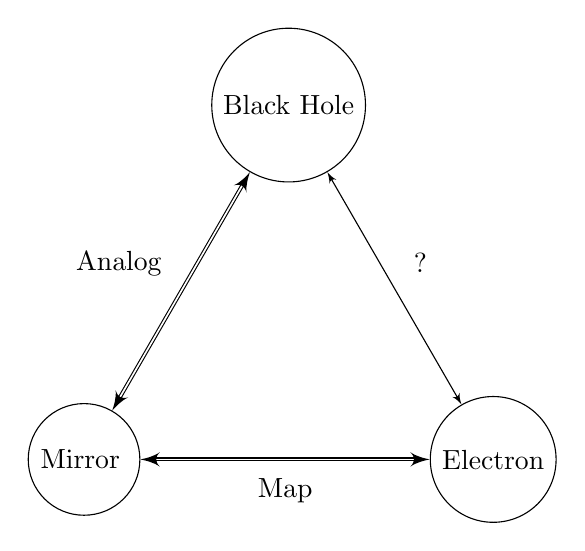
\begin{tikzpicture}
\node[draw,circle] (A) at (90:3) {Black Hole};
\node[draw,circle] (B) at (210:3) {Mirror\;};
\node[draw,circle] (C) at (330:3) {Electron};
\draw[latex'-latex',double] (A) -- node[label=150:Analog,label=330:] {} (B);
\draw[latex'-latex'] (A) -- node[label=30:?,label=210:] {} (C);
\draw[latex'-latex',double] (B) -- node[label=90:,label=270:Map] {} (C);
\end{tikzpicture}

\end{document}